\documentclass[a4paper,12pt]{article} % This defines the style of your paper

\usepackage[top = 2.5cm, bottom = 2.5cm, left = 2.5cm, right = 2.5cm]{geometry} 

% Unfortunately, LaTeX has a hard time interpreting German Umlaute. The following two lines and packages should help. If it doesn't work for you please let me know.
\usepackage[T1]{fontenc}
\usepackage[utf8]{inputenc}
\usepackage{subcaption}

% The following two packages - multirow and booktabs - are needed to create nice looking tables.
\usepackage{multirow} % Multirow is for tables with multiple rows within one cell.
\usepackage{booktabs} % For even nicer tables.
\usepackage{amsmath}
\usepackage{bm}

% As we usually want to include some plots (.pdf files) we need a package for that.
\usepackage{graphicx} 
\usepackage{rotating}
\usepackage{cancel}

% The default setting of LaTeX is to indent new paragraphs. This is useful for articles. But not really nice for homework problem sets. The following command sets the indent to 0.
\usepackage{setspace}
\setlength{\parindent}{0in}

% Package to place figures where you want them.
\usepackage{float}

% The fancyhdr package let's us create nice headers.
\usepackage{fancyhdr}

\usepackage[utf8]{inputenc}
\usepackage[portuguese]{babel}
\usepackage{makecell}
\usepackage{listings}
\usepackage{xcolor}

\definecolor{codegreen}{rgb}{0,0.6,0}
\definecolor{codegray}{rgb}{0.5,0.5,0.5}
\definecolor{codepurple}{rgb}{0.58,0,0.82}
\definecolor{backcolour}{rgb}{0.95,0.95,0.92}

\lstdefinestyle{mystyle}{
    backgroundcolor=\color{backcolour},   
    commentstyle=\color{codegreen},
    keywordstyle=\color{magenta},
    numberstyle=\tiny\color{codegray},
    stringstyle=\color{codepurple},
    basicstyle=\ttfamily\footnotesize,
    breakatwhitespace=false,         
    breaklines=true,                 
    captionpos=b,                    
    keepspaces=true,                 
    numbers=left,                    
    numbersep=5pt,                  
    showspaces=false,                
    showstringspaces=false,
    showtabs=false,                  
    tabsize=2
}
\lstset{style=mystyle}
\renewcommand{\arraystretch}{1.5}

\pagestyle{fancy} % With this command we can customize the header style.

\fancyhf{} % This makes sure we do not have other information in our header or footer.

\lhead{\footnotesize Homework 3}% \lhead puts text in the top left corner. \footnotesize sets our font to a smaller size.

%\rhead works just like \lhead (you can also use \chead)
\rhead{\footnotesize Joana Pimenta, Rodrigo Laia} %<---- Fill in your lastnames.

% Similar commands work for the footer (\lfoot, \cfoot and \rfoot).
% We want to put our page number in the center.
\cfoot{\footnotesize \thepage} 

\begin{document}

\thispagestyle{empty} % This command disables the header on the first page. 

\begin{tabular}{p{15.5cm}} % This is a simple tabular environment to align your text nicely 
{\large \bf Aprendizagem} \\
Instituto Superior Técnico \\ outubro  de 2023  \\ \\ 
\hline % \hline produces horizontal lines.
\\
\end{tabular} % Our tabular environment ends here.

\vspace*{0.3cm} % Now we want to add some vertical space in between the line and our title.

\begin{center} % Everything within the center environment is centered.
	{\Large \bf Homework 3 - Report} % <---- Don't forget to put in the right number
	\vspace{2mm}
	
        % YOUR NAMES GO HERE
	{\bf Joana Pimenta (103730), Rodrigo Laia (102674) } % <---- Fill in your names here!
		
\end{center}  

\vspace{0.4cm}

\section*{Pen and Paper}
\begin{enumerate}

\item 

% \begin{table}[H]
% \centering
% \begin{tabular}{|c|c|c|c|}
% \hline
%  & $y_1$ & $y_2$ & $y_{out}$ \\ \hline
% $x_1$ & 0.7 & -0.3 & 0.8 \\ \hline
% $x_2$ & 0.4 & 0.5 & 0.6 \\ \hline
% $x_3$ & -0.2 & 0.8 & 0.3 \\ \hline
% $x_4$ & -0.4 & 0.3 & 0.3 \\ \hline
% \end{tabular}
% \end{table}


%%%%%%%%%%%%%%%%%% a) %%%%%%%%%%%%%%%%%%%

a) Uma função radial basis permite mapear observações para um novo espaço 
baseando-se na distância entre as observações e os centróides escolhidos.
Neste caso a função radial basis utilizada para transformar as observações foi 
a seguinte:

\begin{equation}
    \phi_j (x) = \exp\left(-\frac{\left\|\vec{x}-c_j\right\|^2}{2}\right)
\end{equation}

O cálculos dos vetores tranformados foi feita através da seguinte fórmula:

\begin{equation}
\vec{\phi_i} = \left( \exp\left(-\frac{\left\|\vec{x}_i-c_1\right\|^2}{2}\right)   , \exp\left(-\frac{\left\|\vec{x}_i-c_2\right\|^2}{2}\right)  , \exp\left(-\frac{\left\|\vec{x}_i-c_3\right\|^2}{2}\right)   \right)
\end{equation}

Assim os vetores transformados obtidos foram:
\begin{equation*}
    \phi_1 = (0.74826,0.74826,0.10127)
\end{equation*}

\begin{equation*}
    \phi_2 = (0.81465,0.27117,0.33121)
\end{equation*}

\begin{equation*}
    \phi_3 = (0.71177,0.09633,0.71177)
\end{equation*}

Para fazer regressão de Ridge é necessário minimizar a função de erro:

\begin{equation}
    E(\vec{w}) = \frac{1}{2} \sum_{i=1}^{n} (z_i - \vec{w}^T \cdot x_i)^2 + \frac{\lambda}{2} ||\vec{w}||^2
\end{equation}

Sendo que isso é equivalente a calcular $\vec{w}$ através da seguinte fórmula:

\begin{equation}
    \vec{w} = (X^T\cdot X + \lambda \cdot I)^{-1} \cdot X^T \cdot \vec{z}
\end{equation}

Uma vez que estamos a trabalhar com uma transformação de espaços, é necessário
calcular a matriz transformada $\Phi$ colocando para cada linha um 1 na primeira
coluna e depois o vetor transformado de cada observação. Utilizamos então as 
fórmulas acima com $\Phi$ no lugar de $X$, assumindo que após a transformação a 
relação entre as variáveis e o target é linear.\\ 

Cálculos intermédios:

\begin{equation*}
    \Phi = 
\begin{bmatrix}
    1 & 0.74826 & 0.74826 & 0.10127 \\ 1 & 0.81465 & 0.27117 & 0.33121 \\ 1 & 0.71177 & 0.09633 & 0.71177 \\ 1 & 0.88250 & 0.16122 & 0.65377
\end{bmatrix}
\end{equation*}

\begin{equation*}
    \Phi^T = \begin{bmatrix}
    1 & 1 & 1 & 1 \\ 0.74826 & 0.81465 & 0.71177 & 0.88250 \\ 0.74826 & 0.27117 & 0.09633 & 0.16122 \\ 0.10127 & 0.33121 & 0.71177 & 0.65377
    \end{bmatrix}
\end{equation*}

\begin{equation*}
    (\Phi^T\cdot \Phi + \lambda \cdot I)^{-1} \cdot \Phi^T = \begin{bmatrix}  0.14105 & 0.35022 & 0.35575 & -0.30185 \\
        -0.09064 & 0.43823 & -0.50361 & 0.53370 \\
         0.99394 & -0.50615  & -0.13690 & -0.16477 \\
        -0.31222 & -0.65246 & 0.72647  &  0.42436 \\ \end{bmatrix}
\end{equation*}

\begin{equation*}
    \vec{w} = \begin{bmatrix}  0.33914 \\ 0.19945 \\ 0.40096 \\ -0.29600 \end{bmatrix}
\end{equation*}

Assim, a regressão de Ridge obtida foi:

\begin{equation*}  
    \hat{z} = 0.33914 + 0.19945 \cdot \phi_1 + 0.40096 \cdot \phi_2 - 0.29600 \cdot \phi_3
\end{equation*}

%%%%%%%%%%%%%%%%%% b) %%%%%%%%%%%%%%%%%%%
b)
Para calcular o RMSE (root mean square error) foi utilizada a seguinte fórmula:

\begin{equation}
    RMSE = \sqrt{\frac{1}{n} \sum_{i=1}^{n} (z_i - \hat{z}_i)^2}
\end{equation}
em que,
\begin{equation}
    \hat{z}_i = \vec{w}^T \cdot \vec{\phi_i}
\end{equation}
 
Targets estimados:
\begin{equation*}
    \hat{z}_1 = 0.75844
\end{equation*}

\begin{equation*}
    \hat{z}_2 = 0.51232
\end{equation*}

\begin{equation*}
    \hat{z}_3 = 0.30905
\end{equation*}

\begin{equation*}
    \hat{z}_4 = 0.38629
\end{equation*}

Assim, o RMSE obtido foi:
\begin{equation*}
    RMSE = 0.06508
\end{equation*}

\item
É importante referir que para este exercício se utilizou a seguinte notação: $L^{\text{camada}}_{observacao}$

As fórmulas utilizadas foram:

\begin{equation}
    \textbf{x}^{[p]} = \phi({W}^{[p]} \cdot \textbf{x}^{[p-1]} + \textbf{b}^{[p]})
\end{equation}

\begin{equation}
    \bm{\delta}^{[p]} = \frac{\partial E}{\partial \textbf{x}^{[p]}} \circ \frac{\partial \textbf{x}^{[p]}}{\partial \textbf{z}^{[p]}} = (\textbf{x}^{[p]} - \mathbf{t}) \circ \phi'(\mathbf{z}^{[p]}) \text{, para a última camada}
\end{equation}    

\begin{equation}
    \bm{\delta}^{[p]} = (\frac{\partial \textbf{z}^{[p+1]}}{\partial \textbf{x}^{[p]}})^T \cdot \bm{\delta}^{[p+1]} \circ \frac{\partial \textbf{x}^{[p]}}{\partial \textbf{z}^{[p]}} = ({W}^{[p+1]})^T \cdot \bm{\delta}^{[p+1]} \circ \phi'(\textbf{z}^{[p]}) \text{, para as outras camadas}
\end{equation}

\begin{equation}
    {W}^{[p]} = {W}^{[p]} - \eta \cdot \frac{\partial E}{\partial {W}^{[p]}} = {W}^{[p]} - \eta \cdot \bm{\delta}^{[p]} \cdot (\textbf{x}^{[p-1]})^T
\end{equation}

\begin{equation}
    \textbf{b}^{[p]} = \textbf{b}^{[p]} - \eta \cdot \frac{\partial E}{\partial \textbf{b}^{[p]}} = \textbf{b}^{[p]} - \eta \cdot \bm{\delta}^{[p]}
\end{equation}

Estas expressões são válidas quando consideramos a squared error loss function.

Dados necessários para começar o algoritmo:

\begin{equation*}
    \textbf{x}^{[0]}_1 = \begin{bmatrix} 1 \\ 1 \\ 1 \\ 1 \end{bmatrix} , \textbf{t}_1 = \begin{bmatrix} -1 \\ 1 \\ -1 \end{bmatrix} , \textbf{x}^{[0]}_2 = \begin{bmatrix} 1 \\ 0 \\ 0 \\ -1 \end{bmatrix} , \textbf{t}_2 = \begin{bmatrix} 1 \\ -1 \\ -1 \end{bmatrix}
\end{equation*}

\begin{equation*}
    W^{[1]} = \begin{bmatrix} 1 & 1 & 1 & 1 \\ 1 & 1 & 2 & 1 \\ 1 & 1 & 1 & 1 \end{bmatrix} , \textbf{b}^{[1]} = \begin{bmatrix} 1 \\ 1 \\ 1 \end{bmatrix}
\end{equation*}

\begin{equation*}
    W^{[2]} = \begin{bmatrix} 1 & 4 & 1 \\  1 & 1 & 1 \end{bmatrix} , \textbf{b}^{[2]} = \begin{bmatrix} 1 \\ 1 \end{bmatrix}
\end{equation*}

\begin{equation*}
    W^{[3]} = \begin{bmatrix} 1 & 1 \\ 3 & 1 \\ 1 & 1 \end{bmatrix} , \textbf{b}^{[3]} = \begin{bmatrix} 1 \\ 1 \\ 1 \end{bmatrix}
\end{equation*}

\begin{equation*}
    \phi = tanh(0.5x -2) \text{, } \phi' = 0.5 * (1 - tanh^2(0.5x -2))
\end{equation*}

Guia de rede considerado:

\begin{figure}[H]
    \centering
    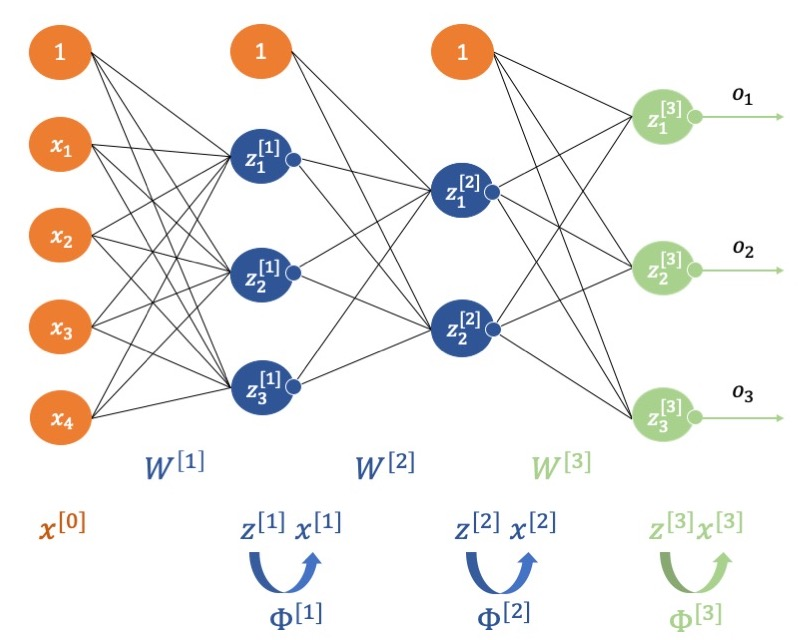
\includegraphics[width=0.7\textwidth]{rede.jpg}
\end{figure}

\begin{figure}[H]
    \centering
    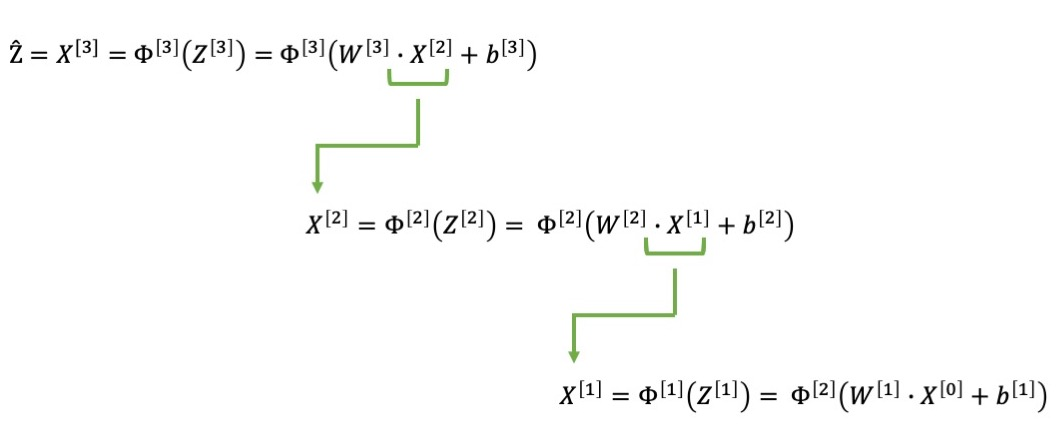
\includegraphics[width=0.9\textwidth]{equacoes.jpg}
\end{figure}

Primeiro é necessário realizar (forward) propagation para obter os valores das observações:

- Para a primeira observação:

\begin{equation*}
    \textbf{z}^{[1]}_1 = W^{[1]} \cdot \textbf{x}^{[0]}_1 + \textbf{b}^{[1]} = \begin{bmatrix} 5 \\ 6 \\ 5 \end{bmatrix} \implies \textbf{x}^{[1]}_1 = \phi(\textbf{z}^{[1]}_1)= \begin{bmatrix} 0.46212 \\ 0.76159 \\ 0.46212 \end{bmatrix}
\end{equation*}

\begin{equation*}
    \textbf{z}^{[2]}_1 = W^{[2]} \cdot \textbf{x}^{[1]}_1 + \textbf{b}^{[2]} = \begin{bmatrix} 4.97061 \\ 2.68583 \end{bmatrix} \implies \textbf{x}^{[2]}_1 = \phi(\textbf{z}^{[2]}_1)= \begin{bmatrix} 0.45048 \\ -0.57642 \end{bmatrix}
\end{equation*}

\begin{equation*}
    \textbf{z}^{[3]}_1 = W^{[3]} \cdot \textbf{x}^{[2]}_1 + \textbf{b}^{[3]} = \begin{bmatrix} 0.87406 \\ 1.77503 \\ 0.87406 \end{bmatrix} \implies \textbf{x}^{[3]}_1 = \phi(\textbf{z}^{[3]}_1)= \begin{bmatrix} -0.91590 \\ -0.80494\\ -0.91590 \end{bmatrix}
\end{equation*}

- Para a segunda observação:

\begin{equation*}
    \textbf{z}^{[1]}_2 = W^{[1]} \cdot \textbf{x}^{[0]}_2 + \textbf{b}^{[1]} = \begin{bmatrix} 1 \\ 1 \\ 1 \end{bmatrix} \implies \textbf{x}^{[1]}_2 = \phi(\textbf{z}^{[1]}_2)= \begin{bmatrix} -0.90515 \\ -0.90515 \\ -0.90515 \end{bmatrix}
\end{equation*}

\begin{equation*}
    \textbf{z}^{[2]}_2 = W^{[2]} \cdot \textbf{x}^{[1]}_2 + \textbf{b}^{[2]} = \begin{bmatrix} -4.43089 \\ -1.71545 \end{bmatrix} \implies \textbf{x}^{[2]}_2 = \phi(\textbf{z}^{[2]}_2)= \begin{bmatrix} -0.99956 \\ -0.99343 \end{bmatrix}
\end{equation*}

\begin{equation*}
    \textbf{z}^{[3]}_2 = W^{[3]} \cdot \textbf{x}^{[2]}_2 + \textbf{b}^{[3]} = \begin{bmatrix} -0.99300 \\ -2.99212 \\ -0.99300 \end{bmatrix} \implies \textbf{x}^{[3]}_2 = \phi(\textbf{z}^{[3]}_2)= \begin{bmatrix} -0.98652 \\ -0.99816\\ -0.98652 \end{bmatrix}
\end{equation*}

Depois é necessário realizar (backward) propagation dos erros da última camada para a primeira:

- Para a primeira observação:

\begin{equation*}
    \bm{\delta}^{[3]}_1 = (\textbf{x}^{[3]}_1 - \textbf{t}_1) \circ \phi'(\textbf{z}^{[3]}_1) = \begin{bmatrix} -0.00678\\ -0.31773 \\ -0.00678 \end{bmatrix}
\end{equation*}

\begin{equation*}
    \bm{\delta}^{[2]}_1 = (W^{[3]})^T \cdot \bm{\delta}^{[3]}_1 \circ \phi'(\textbf{z}^{[2]}_1) = \begin{bmatrix} -0.37448\\ -0.10156 \end{bmatrix}
\end{equation*}

\begin{equation*}
    \bm{\delta}^{[1]}_1 = (W^{[2]})^T \cdot \bm{\delta}^{[2]}_1 \circ \phi'(\textbf{z}^{[1]}_1) = \begin{bmatrix} -0.18719 \\ -0.33587 \\ -0.18719 \end{bmatrix}
\end{equation*}

- Para a segunda observação:

\begin{equation*}
    \bm{\delta}^{[3]}_2 = (\textbf{x}^{[3]}_2 - \textbf{t}_2) \circ \phi'(\textbf{z}^{[3]}_2) = \begin{bmatrix} -2.65961\cdot 10^{-2} \\ 3.36962\cdot 10^{-6} \\ 1.80463\cdot 10^{-4} \end{bmatrix}
\end{equation*}

\begin{equation*}
    \bm{\delta}^{[2]}_2 = (W^{[3]})^T \cdot \bm{\delta}^{[3]}_2 \circ \phi'(\textbf{z}^{[2]}_2) = \begin{bmatrix} -1.15093\cdot 10^{-5} \\ -1.72899 \cdot 10^{-4} \end{bmatrix}
\end{equation*}

\begin{equation*}
    \bm{\delta}^{[1]}_2 = (W^{[2]})^T \cdot \bm{\delta}^{[2]}_2 \circ \phi'(\textbf{z}^{[1]}_2) = \begin{bmatrix} -1.66619\cdot 10^{-5} \\ -1.97816 \cdot 10^{-5} \\ -1.66193\cdot 10^{-5} \end{bmatrix}
\end{equation*}

Por fim é necessário atualizar os pesos e os bias. Como estamos a realizar um batch gradient descent update (com learning rate igual a 0.1), a expressão para os pesos atualizados é:

\begin{equation}
    W^{[p]} = W^{[p]} - \eta \cdot (\bm{\delta}^{[p]}_1 \cdot (\textbf{x}^{[p-1]}_1)^T + \bm{\delta}^{[p]}_2 \cdot (\textbf{x}^{[p-1]}_2)^T)
\end{equation}

Assim, os pesos e os bias atualizados foram:

\begin{equation*}
    W^{[1]} = W^{[1]} - 0.1 \cdot (\bm{\delta}^{[1]}_1 \cdot (\textbf{x}^{[0]}_1)^T + \bm{\delta}^{[1]}_2 \cdot (\textbf{x}^{[0]}_2)^T) = \begin{bmatrix} 1.01872 & 1.01872 & 1.01872 & 1.01872 \\
                                                                                                                            1.03359 & 1.03359 & 2.03359 & 1.03359 \\
                                                                                                                            1.01872 & 1.01872 & 1.01872 & 1.01872 \end{bmatrix}
\end{equation*}

\begin{equation*}
    \textbf{b}^{[1]} = \textbf{b}^{[1]} - 0.1 \cdot (\bm{\delta}^{[1]}_1 + \bm{\delta}^{[1]}_2) = \begin{bmatrix} 1.01872 \\ 1.03359 \\ 1.01872 \end{bmatrix}
\end{equation*}

\begin{equation*}
    W^{[2]} = W^{[2]} - 0.1 \cdot (\bm{\delta}^{[2]}_1 \cdot (\textbf{x}^{[1]}_1)^T + \bm{\delta}^{[2]}_2 \cdot (\textbf{x}^{[1]}_2)^T) = \begin{bmatrix} 1.01730 & 4.02852 & 1.01730 \\
                                                                                                                            1.00468 & 1.00772 & 1.00468 \end{bmatrix}
\end{equation*}

\begin{equation*}
    \textbf{b}^{[2]} = \textbf{b}^{[2]} - 0.1 \cdot (\bm{\delta}^{[2]}_1 + \bm{\delta}^{[2]}_2) = \begin{bmatrix} 1.03745 \\ 1.01017 \end{bmatrix}
\end{equation*}

\begin{equation*}
    W^{[3]} = W^{[3]} - 0.1 \cdot (\bm{\delta}^{[3]}_1 \cdot (\textbf{x}^{[2]}_1)^T + \bm{\delta}^{[3]}_2 \cdot (\textbf{x}^{[2]}_2)^T) = \begin{bmatrix} 0.99704 & 0.99775 \\
                                                                                                                            3.01431 & 0.98169 \\
                                                                                                                            0.99971 & 1.00041 \end{bmatrix}
\end{equation*}

\begin{equation*}
    \textbf{b}^{[3]} = \textbf{b}^{[3]} - 0.1 \cdot (\bm{\delta}^{[3]}_1 + \bm{\delta}^{[3]}_2) = \begin{bmatrix} 1.00198 \\ 1.03177 \\ 0.99930 \end{bmatrix}
\end{equation*}

Para facilitar a resolução deste exercício, críamos um código em \textit{Python} para 
realizar os cálculos necessários utilizando a biblioteca \textit{numpy}.\\

\begin{lstlisting}[language=Python]
import numpy as np 

### MLP ###

x1 = np.array([[1], [1], [1], [1]])
x2 = np.array([[1], [0], [0], [-1]])

w1 = np.array([[1, 1, 1, 1], [1, 1, 2, 1], [1, 1, 1, 1]])
print('w1: \n', w1)
b1 = np.array([[1], [1], [1]])
print('b1: \n', b1)
t1 = np.array([[-1], [1], [-1]])
print('t1: \n', t1)

w2 = np.array([[1, 4, 1], [1, 1, 1]])
print('w2: \n', w2)
b2 = np.array([[1], [1]])
print('b2: \n', b2)
t2 = np.array([[1], [-1], [-1]])
print('t2: \n', t2)

w3 = np.array([[1, 1], [3, 1], [1, 1]])
print('w3: \n', w3)
b3 = np.array([[1], [1], [1]])
print('b3: \n', b3)

def phi(x):
    return np.tanh(0.5 * x - 2)

def phi_prime(x):
    return 0.5 * (1 - np.tanh(0.5 * x - 2) ** 2)

# x1_p and x2_p being p the index of the layer

### first observation ###

z1_1 = np.dot(w1, x1) + b1
print('z1_1: \n', z1_1)
x1_1 = phi(z1_1)
print('x1_1: \n', x1_1)

z1_2 = np.dot(w2, x1_1) + b2
print('z1_2: \n', z1_2)
x1_2 = phi(z1_2)
print('x1_2: \n', x1_2)

z1_3 = np.dot(w3, x1_2) + b3
print('z1_3: \n', z1_3)
x1_3 = phi(z1_3) 
print('x1_3: \n', x1_3)

delta1_3 = (x1_3 - t1) * phi_prime(z1_3)
print('delta1_3: \n', delta1_3)

delta1_2 = np.dot(w3.transpose(), delta1_3) * phi_prime(z1_2)
print('delta1_2: \n', delta1_2)

delta1_1 = np.dot(w2.transpose(), delta1_2) * phi_prime(z1_1)
print('delta1_1: \n', delta1_1)

### second observation ###

z2_1 = np.dot(w1, x2) + b1
print('z2_1: \n', z2_1)
x2_1 = phi(z2_1)
print('x2_1: \n', x2_1)

z2_2 = np.dot(w2, x2_1) + b2
print('z2_2: \n', z2_2)
x2_2 = phi(z2_2)
print('x2_2: \n', x2_2)

z2_3 = np.dot(w3, x2_2) + b3
print('z2_3: \n', z2_3)
x2_3 = phi(z2_3)
print('x2_3: \n', x2_3)

delta2_3 = (x2_3 - t2) * phi_prime(z2_3)
print('delta2_3: \n', delta2_3)

delta2_2 = np.dot(w3.transpose(), delta2_3) * phi_prime(z2_2)
print('delta2_2: \n', delta2_2)

delta2_1 = np.dot(w2.transpose(), delta2_2) * phi_prime(z2_1)
print('delta2_1: \n', delta2_1)

### derivatives ###
dE1_dw1 = np.dot(delta1_1, x1.transpose())
print('dE1_dw1: \n', dE1_dw1)

dE2_dw1 = np.dot(delta2_1, x2.transpose())
print('dE2_dw1: \n', dE2_dw1)

dE1_dw2 = np.dot(delta1_2, x1_1.transpose())
print('dE1_dw2: \n', dE1_dw2)

dE2_dw2 = np.dot(delta2_2, x2_1.transpose())
print('dE2_dw2: \n', dE2_dw2)

dE1_dw3 = np.dot(delta1_3, x1_2.transpose())
print('dE1_dw3: \n', dE1_dw3)

dE2_dw3 = np.dot(delta2_3, x2_2.transpose())
print('dE2_dw3: \n', dE2_dw3)

### final weights ###

w1_new = w1 - 0.1 * (dE1_dw1 + dE2_dw1)
print('w1_new: \n', w1_new)

w2_new = w2 - 0.1 * (dE1_dw2 + dE2_dw2)
print('w2_new: \n', w2_new)

w3_new = w3 - 0.1 * (dE1_dw3 + dE2_dw3)
print('w3_new: \n', w3_new)

### final biases ###

b1_new = b1 - 0.1 * (delta1_1 + delta2_1)
print('b1_new: \n', b1_new)

b2_new = b2 - 0.1 * (delta1_2 + delta2_2)
print('b2_new: \n', b2_new)

b3_new = b3 - 0.1 * (delta1_3 + delta2_3)
print('b3_new: \n', b3_new)
\end{lstlisting}

\end{enumerate}

\clearpage

\section*{Programming - Código Python e Resultados Obtidos}

\begin{enumerate}

\item Utilizamos um training-test split de 80-20, ou seja 80\% dos dados foram utilizados para treinar o modelo e 20\% para testá-lo.\\ 
Usando 10 regressores MLP com as características especificadas no enunciado e com sementes de 1 a 10, 
previmos o output para as observações de teste e calculamos os resíduos através da seguinte fórmula.

\begin{equation}
    \text{residual} = (z - \hat{z})
\end{equation}

O histograma dos módulos dos resíduos dos 10 MLP's (com sementes de 1 a 10) encontra-se representado na seguinte figura:

\begin{figure}[H]
    \centering
    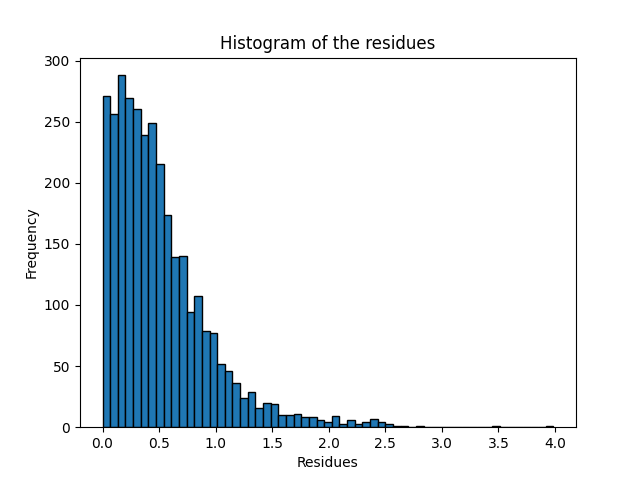
\includegraphics[width=0.7\textwidth]{ex1_histogram.png}
\end{figure}

Observando o histograma, conclui-se que a frequência diminui significativamente 
com o crescimento do valor absoluto dos resíduos. Isto significa que a maior parte
da diferença entre o valor real e o valor previsto pelo MLP é pequena, logo a previsão
dos MLP's em geral é bastante boa.\\

Código Utilizado:

\begin{lstlisting}[language=Python]
import pandas as pd, numpy as np
import matplotlib.pyplot as plt
from sklearn.model_selection import train_test_split
from sklearn.neural_network import MLPRegressor
from sklearn.metrics import mean_absolute_error

# Reading the csv file
df = pd.read_csv('Homework3/winequality-red.csv')
# Separating the variables from the target
variables = df.drop("quality", axis= 1)
target = df['quality']

# Training Test Split
variables_train, variables_test, target_train, target_test= train_test_split(variables, target, 
                                                                            train_size=0.8, random_state=0)

######### Exercise 1 ##########
residues = np.array([])

for i in range(1, 11):
    # Learn the MLP regressor 
    mlp = MLPRegressor(hidden_layer_sizes=(10,10), activation='relu', early_stopping=True, validation_fraction=0.2, random_state=i)
    #Predict output
    y_pred = mlp.fit(variables_train,target_train).predict(variables_test)
    #Calculate residues
    residue = abs(target_test - y_pred)
    residue = residue.to_numpy()
    residues = np.append(residues, residue)
    
#Plot all the residues
plt.hist(residues, edgecolor='black',bins='auto')
plt.title('Histogram of the residues')
plt.xlabel('Residues')
plt.ylabel('Frequency')
plt.savefig('ex1_histogram.png')
plt.show()
    
\end{lstlisting}

\item Uma vez que sabemos que a qualidade do vinho tem de ser um inteiro entre 
1 e 10 podemos arredondar os valores previstos pelo MLP para o inteiro mais próximo (arredondamento)
e transformar os valores menores que 1 em 1 e os maiores que 10 em 10 (limitação).\\
Para comparar o desempenho do MLP antes e depois destes processos, comparamos os MAE's obtidos. 
\\ Consideramos que o valor do MAE é a média dos valores dos MAE's dos 10 MLP's com sementes de 1 a 10.\\
A fórmula que usamos para calcular cada um destes 10 MAE's foi:

\begin{equation}
    MAE = \frac{1}{n} \sum_{i=1}^{n} | z_i - \hat{z}_i |
\end{equation}

Os valores obtidos foram os seguintes:

\begin{table}[H]
\centering
\begin{tabular}{|c|c|}
\hline
Processo aplicado & MAE \\ \hline
Nenhum & 0.50972 \\ \hline
Arredondamento & 0.43875 \\ \hline
Limitação & 0.50972 \\ \hline
Arredondamento e limitação & 0.43875 \\ \hline
\end{tabular}
\end{table}

Assim, conclui-se que para este dataset o arredondamento tem um feito positivo no desempenho do MLP, enquanto que a limitação não tem qualquer efeito.\\

Código Utilizado:

\begin{lstlisting}[language=Python]
########## Exercise 2 ##########
# Round and bound the predictions
mae_array = np.array([])
mae_bounded_array = np.array([])
mae_rounded_array = np.array([])
mae_rounded_and_bounded_array = np.array([])

for i in range(1, 11):
    # Learn the MLP regressor 
    mlp = MLPRegressor(hidden_layer_sizes=(10,10), activation='relu', early_stopping=True, validation_fraction=0.2, random_state=i)

    #Calculate MAE
    y_pred = mlp.fit(variables_train,target_train).predict(variables_test)
    mae = mean_absolute_error(target_test, y_pred)
    #mae = np.mean(abs(target_test - y_pred))
    mae_array = np.append(mae_array, mae)
    print(mae)
    #Calculate MAE - rounded
    y_pred_rounded = np.round(y_pred)
    mae_rounded = np.mean(abs(target_test - y_pred_rounded))
    mae_rounded_array = np.append(mae_rounded_array, mae_rounded)
    
    #Calculate MAE - bounded
    y_pred_bounded = np.clip(y_pred, a_min=1, a_max=10)
    mae_bounded = np.mean(abs(target_test - y_pred_bounded))
    mae_bounded_array = np.append(mae_bounded_array, mae_bounded)

    ##Calculate MAE - rounded and bounded
    y_pred_rounded_and_bounded = np.clip(y_pred_rounded, a_min=1, a_max=10)
    mae_rounded_and_bounded = np.mean(abs(target_test - y_pred_rounded_and_bounded))
    mae_rounded_and_bounded_array = np.append(mae_rounded_and_bounded_array, mae_rounded_and_bounded)

mean_mae = np.mean(mae_array)
mean_mae_rounded = np.mean(mae_rounded_array)
mean_mae_bounded = np.mean(mae_bounded_array)
mean_mae_rounded_and_bounded = np.mean(mae_rounded_and_bounded_array)

# Print the results
print('MAE (not rounded and not bounded): ', mean_mae)
print('MAE (rounded): ', mean_mae_rounded)
print('MAE (bounded): ', mean_mae_bounded)
print('MAE (rounded and bounded): ', mean_mae_rounded_and_bounded)
\end{lstlisting}

\item Até agora foram considerados MLP's com early stopping. Neste exercício vamos
ver qual é o efeito do número máximo de iterações no desempenho do MLP, avaliado através do RMSE.
Assim foram considerados 4 MLP's com números máximos de iterações iguais a 20, 50, 100 e 200. 
Da mesma maneira que antes, o RMSE considerado foi a média dos 10 RMSE's de cada ums dos modelos com sementes de 1 a 10. 
No gráfico seguinte encontra-se representado o RMSE em função do número máximo de iterações.\\ \\

\begin{figure}[H]
\centering
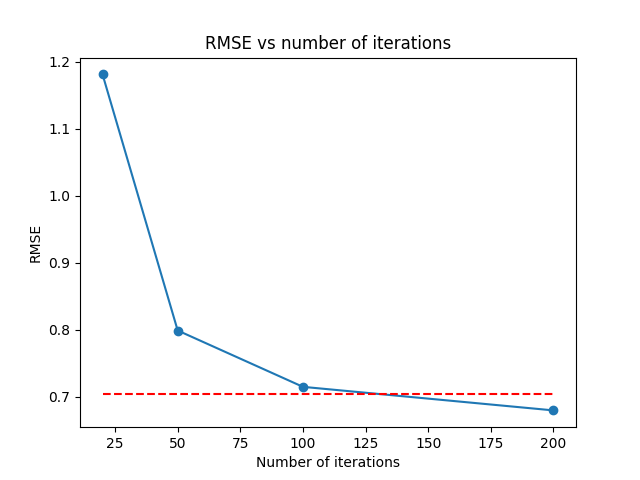
\includegraphics[width=0.7\textwidth]{ex3_rmse.png}
\end{figure}

Observando o gráfico, conclui-se que o RMSE diminui significativamente com o aumento do número máximo de iterações.
No entanto, essa diminuição abranda à medida que se aumenta o número máximo de iterações.\\

Código utilizado:

\begin{lstlisting}[language=Python]
########## Exercise 3 ##########
# Calculate the RMSE for the old MLP regressor
sum_rmse_old = 0
for i in range(1, 11):
    #Learn the old MLP regressor
    mlp = MLPRegressor(hidden_layer_sizes=(10,10), activation='relu', early_stopping=True, validation_fraction=0.2, random_state=i)
    #Predict old output
    y_pred_old = mlp.fit(variables_train,target_train).predict(variables_test)
    #Calculate old RMSE
    rmse = np.sqrt(np.mean((target_test - y_pred_old) ** 2))
    sum_rmse_old += rmse

average_rmse_old = np.mean(sum_rmse_old/10)

# Calculate the RMSE for each number of iterations
new_rmse_array = []
iter_array = [20,50,100,200]
for iter in iter_array:
    y_pred_new = np.zeros(len(target_test))
    sum_rmse_new = 0
    for i in range(1, 11):
        # Learn the new MLP regressor 
        mlp = MLPRegressor(hidden_layer_sizes=(10,10), activation='relu', max_iter = iter, random_state=i)
        #Predict new output
        y_pred_new = mlp.fit(variables_train,target_train).predict(variables_test)
        #Calculate new RMSE
        rmse = np.sqrt(np.mean((target_test - y_pred_new) ** 2))
        sum_rmse_new += rmse
    #Append new RMSE
    new_rmse_array += [sum_rmse_new/10]

def const(x): return average_rmse_old

# Plot the RMSE
plt.plot(iter_array, new_rmse_array, '-o', label='Different max iteration MLP')
plt.hlines(average_rmse_old, xmin=min(iter_array), xmax=max(iter_array), colors='r', linestyles='dashed', label = 'Early stopping MLP')
plt.xlabel('Number of iterations') 
plt.ylabel('RMSE')
plt.title('RMSE vs number of iterations')
plt.legend()
plt.savefig('ex3_rmse.png')
plt.show()
\end{lstlisting}

\item De um modo geral, o MLP com early stopping tem um desempenho melhor em comparação com um número fixo de iterações. Isto é, o RMSE obtido com early stopping é menor do que o RMSE obtido com um número fixo de iterações (20, 50 e 100).
Para o número máximo de iterações igual a 200, o RMSE obtido com early stopping é maior do que o RMSE obtido com um número fixo de iterações. No entanto, a diferença entre os dois RMSE's é muito pequena.

Early stopping é uma técnica utilizada para combater o overfitting. No entanto, pode impedir que o modelo alcance o seu potencial total de ajuste se o critério de paragem utilizado não for o mais adequado (por ser demasiado elevado, por exemplo).

Também é importante referir que definir um número fixo de iterações pode ser ineficiente, já que o modelo pode não precisar de tantas iterações para convergir para uma solução aceitável. 

O early stopping a 20\% é um critério de paragem que fornece um certo nível de flexibilidade no treino do modelo. Ele permite que o treino continue até que o modelo comece a demonstrar um claro sinal de overfitting, mas também evita que seja encerrado prematuramente devido a flutuações no erro.

No caso específico dos dados em questão, concluímos que o melhor critério de paragem a utilizar seria o early stopping, uma vez que apesar de o RMSE obtido com early stopping ser maior do que o RMSE obtido com um número fixo de iterações (200), a diferença entre os dois RMSE's é desprezável. 
Assim, o early stopping é o critério de paragem que permite obter o melhor desempenho do modelo, uma vez que evita o overfitting e é significativamente mais eficiente do que um número fixo de iterações.\\

\end{enumerate}

\end{document}
